\documentclass[tikz]{standalone}
\usepackage{amsmath}
\usepackage{pgfplots}
\usepackage{csvsimple}

\usetikzlibrary{arrows,intersections,math}

\begin{document}
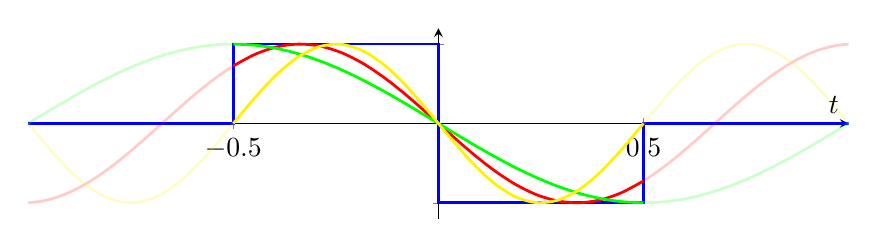
\begin{tikzpicture}
	\begin{axis}[width=12cm, height=4cm, xmin=-1, xmax=1, ymin=-1.2, ymax=1.2,
		axis lines=middle, ytick={-2}, extra y ticks={-1, 1}, extra y tick labels={}, xtick={-0.5, 0.5},
		xlabel=$t$]
		\addplot[mark=none, color=blue, line width=1pt] coordinates 
		{(-2, 0 ) (-0.5, 0) (-0.5, 1) (0, 1) (0, -1) (0.5, -1) (0.5, 0) (2, 0)};
		
		\addplot[domain=-1.0:-0.5, samples=20, smooth, color=red, opacity=0.2, line width=1pt] {-sin(360*x*0.742)};
		\addplot[domain=-0.5: 0.5, samples=20, smooth, color=red, opacity=1.0, line width=1pt] {-sin(360*x*0.742)};
		\addplot[domain= 0.5: 1.0, samples=20, smooth, color=red, opacity=0.2, line width=1pt] {-sin(360*x*0.742)};
		
		\addplot[domain=-1.0:-0.5, samples=20, smooth, color=green, opacity=0.2, line width=1pt] {-sin(360*x*0.5)};
		\addplot[domain=-0.5: 0.5, samples=20, smooth, color=green, opacity=1.0, line width=1pt] {-sin(360*x*0.5)};
		\addplot[domain= 0.5: 1.0, samples=20, smooth, color=green, opacity=0.2, line width=1pt] {-sin(360*x*0.5)};
		
		\addplot[domain=-1.0:-0.5, samples=20, smooth, color=yellow, opacity=0.2, line width=1pt] {-sin(360*x*1.0)};
		\addplot[domain=-0.5: 0.5, samples=20, smooth, color=yellow, opacity=1.0, line width=1pt] {-sin(360*x*1.0)};
		\addplot[domain= 0.5: 1.0, samples=20, smooth, color=yellow, opacity=0.2, line width=1pt] {-sin(360*x*1.0)};
	\end{axis}

\end{tikzpicture}
\end{document}
